\section{Evaluation} \label {chapter:evaluation}

\subsection{Succes rate of the network}
Using the 1 hidden layer and 100 hidden neurons the error rate in the validation set was down to 2.67\% after 1000 epochs which corresponds to 30 errors of the (7854/7) targets in the validation set. In the test set the error percentage was 85.38\% with 958 errors. To show the dispersion of the errors a confusion plot was made from the outputs and targets using Matlab. The confusion matrix is show in \cref{confusion_matrix} and a plot of the values is show in \cref{confusion_plot}.


\begin{figure}[!h]
\begin{center}
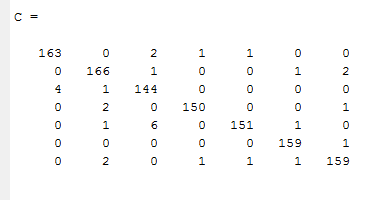
\includegraphics[width=10cm]{testresults/confusionmatrix.png}
\caption{Confusion matrix}
\label{confusion_matrix}
\end{center}
\end{figure}
\FloatBarrier

\begin{figure}[!h]
\begin{center}
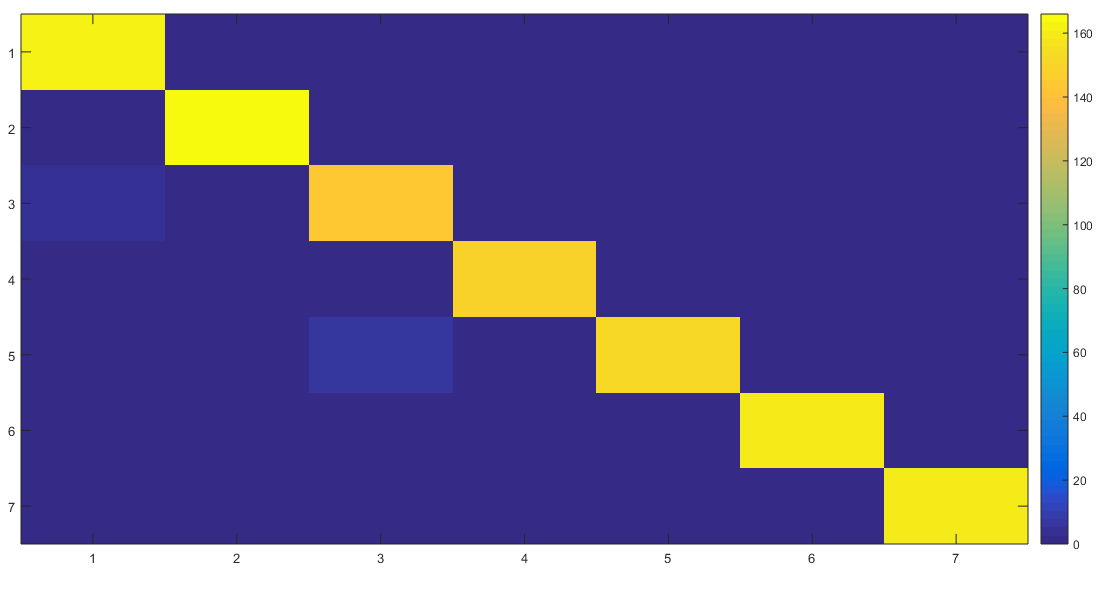
\includegraphics[width=10cm]{testresults/confusionplot.png}
\caption{Confusion plot}
\label{confusion_plot}
\end{center}
\end{figure}
\FloatBarrier

From the matrix and plot it can be concluded that the trained network works quite well on the validation set. The few errors that exist are somewhat evenly distributed over the whole set. Output number 3 has the highest error rate of 5.88\% with 9 error values from the 144+9=153 values.

